\section{Introduction}

As technology ventures deeper into the nanoscale, accurate theoretical models
of electronic bahavior at this scale become vital. For many cases, approaches
which rely on approximate DFT for electronic structure will suffice, however,
in the case of moderate or strong electronic correlation, methods from the
field of Quantum Chemistry become unavoidable.

When treating systems connected to semi-infinite leads, further problems arise:
device states can couple to the continuum and become complex resonances
described by Siegert wave functions. Conventional approaches to the description
of these systems model this coupling by inserting a complex self-energy term
$\Sigma$ into the Hamiltonian. This term however contains a dependence on the
single-particle energy, making it impractical for use with wave function
methods.

In earlier work~\cite{henderson}, a method was outlined in which an
energy-dependent self-energy is mapped to an energy-independent Complex
Absorbing Potential (CAP), which, when added to the Hamiltonian, can be used
in a many-body treatment of the system. Here we present a continuation of that
work, applying the method to a chain of atoms with interacting electrons.
Different levels of correlation are explored by varying the threshold
parameter for Configuration State Functions (CSFs) in the Configuration
Interaction (CI) calculation.

The rest of this paper is organized as follows: in section~\ref{sec:method}, we
cover the methods used in this work, both for constructing the CAP and for
solving the resulting complex symmetric many-body problem. In
section~\ref{sec:results} we present some results of applying the formalism to
a simple atomic chain system. Finally, section~\ref{sec:discussion} contains a
discussion of the results, as well as conclusions and further perspectives.


\section{Method}
\label{sec:method}

\subsection{Model System}
\label{subsec:modelsystem}

The system we studied consists of a simple atomic chain with interatomic
separation of 0.28 nm (?), intended to mirror the system studied experimentally
in [science paper?] (See figure~\ref{fig:chaincapdevice}). Two interatomic
spacings are made larger than the others, to delineate a ``device'' between two
leads. This spacing determines the degree to which the device states couple to
the leads, and variation of the spacing allows us to explore different coupling
regimes.

\begin{figure}
	\begin{center}
		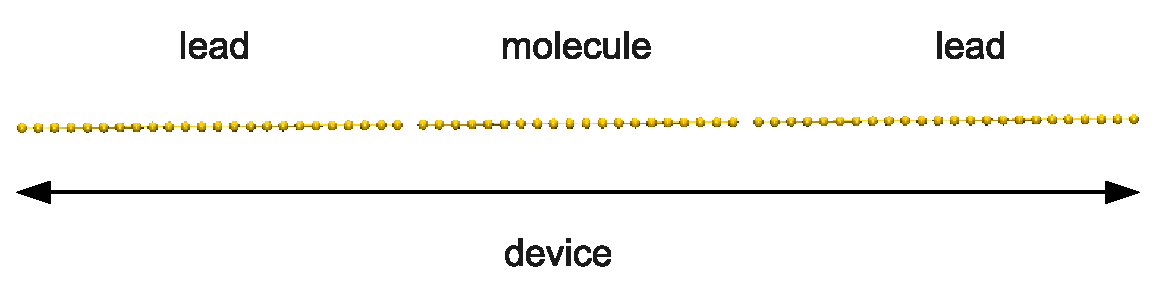
\includegraphics[width=0.9\linewidth]{figures/chaincapdevice}
	\end{center}
	\caption{Model system studied in this work. The device consists of 24
	Gold atoms, while the leads (not fully shown to accentuate the
	device-lead gaps) consist of 20 atoms each.}
	\label{fig:chaincapdevice}
\end{figure}

For comparison purposes, the transmission spectrum of this system was
calculated in the NEGF formalism using the TIMES~\cite{times} code. The
objective is to model the peaks of this spectrum with Lorentzian curves for
which the peak location and peak width are extracted from the real and
imaginary parts, respectively, of the complex eigenvalues obtained by
diagonalization of the Hamiltonian which includes a complex symmetric CAP.

\subsection{Complex Absorbing Potential}
\label{subsec:CAP}

The CAP was constructed as follows (for a detailed description, see~
\cite{henderson}):

[irene can explain this better?]

\subsection{Complex Monte Carlo Configuration Interaction}

The CI calculations were performed using a version of the Monte Carlo
Configuration Interaction (MCCI) program, modified according to the orthogonal
projection method outlined in~\cite{tarantelli_csd} to solve the complex
symmetric generalized eigenvalue problem that results when a CAP is introduced
into the Hamiltonian. To explore the effect of electron correlation on the
shifts and broadenings, we ran calculations with different values of the
threshold parameter $cmin$, which acts as a lower limit for the expansion
coefficients of CSFs which are to be included in the final expansion. Only
those CSFs which excited into or from states localized in the device (as
opposed to the part of the leads which is included in the device region) were
considered, since we wanted to explore only excitations of the actual device.

\section{Results}
\label{sec:results}

\subsection{Single-Particle Picture}
\label{subsec:SingleParticle}

As a validation of the CAP approach, we would first like to see whether the
CAP as generated according to the description of section~\ref{subsec:CAP} gives
the correct complex single-particle eigenvalues, i.e. whether the selected
self-consistent solutions of the Dyson equation provide an accurate picture of
the resonances in the device region. To this end, we convert the complex
eigenvalues of $\um{H} + \um{W}$ to Lorentzian broadened peaks according to

\begin{equation}
	f(\varepsilon;E_{res})
	= \frac{\Gamma^2}{(\varepsilon - \operatorname{Re}(E_{res}))^2 + \Gamma^2}
	\label{eq:lobro}
\end{equation}

where $\Gamma = 2 \times \operatorname{Im}(E_{res})$ is the broadening
associated with the eigenvalue, and compare to a transmission spectrum of the
device obtained using the self-energy in the NEGF formalism. Such a comparison
is shown in figure~\ref{fig:lobro-hwevals}, with good agreement between the
two. (The agreement is also obtained outside the plotted range.)

\begin{figure}
	\begin{center}
		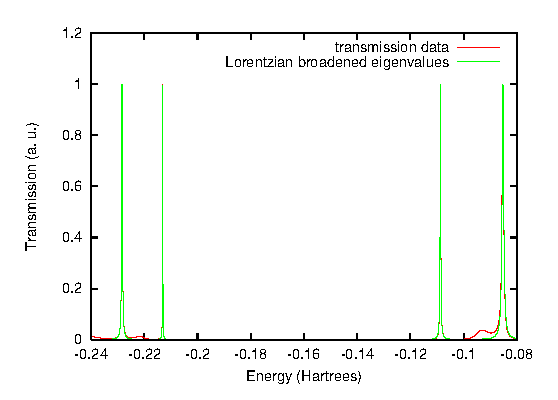
\includegraphics[width=0.9\linewidth]{figures/4evals}
	\end{center}
	\caption{Comparison of transmission data (red) with Lorentzian
	broadened complex eigenvalues of $\um{H}_0 + \um{W}$ (green) for a
	model system as described in section~\ref{subsec:modelsystem}, with
	device-lead gap of 0.45 nm. Transmission data was obtained from NEGF
	calculations with the TIMES program~\cite{times}.}
	\label{fig:lobro-hwevals}
\end{figure}

\subsection{Single Determinant}
\label{subsec:SingleDeterminant}

The next step is to pass to the many-body picture, initially representing the
wave function of the $N$ electron system as a single Slater determinant. The
quasiparticle peaks in the transmission spectrum are approximated by taking
differences of many-body energies: $E^N - E^{N-1}$ yields the HOMO, while
likewise $E^{N+1} - E^N$ yields the LUMO (other quasiparticle levels can be
obtained by taking differences of excited many-body energies). The peaks for
the HOMO and LUMO of the system obtained in this way are plotted in figure
\ref{fig:nobranch}.

\begin{figure}
	\begin{center}
		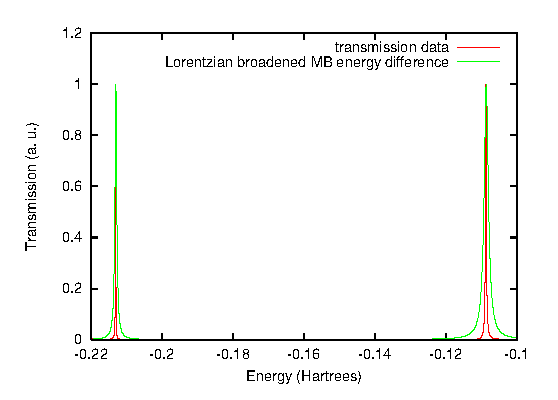
\includegraphics[width=0.9\linewidth]{figures/nobranch}
	\end{center}
	\caption{HOMO and LUMO quasiparticle levels from
	figure~\ref{fig:lobro-hwevals} with the }
	\label{fig:nobranch}
\end{figure}

\subsection{Single Excitations}
\label{subsec:singles}

The next step is to include, for each state, the reference determinant plus all
its single excitations. By Thouless' theorem~\cite{Thouless}, the wave function
obtained in this way would still be describable as a single determinant (and
thus, by definition, contain no correlation), but by adding degrees of freedom
to the system, a degree of self-consistency is attained. The results for the
HOMO and LUMO quasiparticle levels are plotted in figure~\ref{fig:singles}.

\begin{figure}
	\begin{center}
		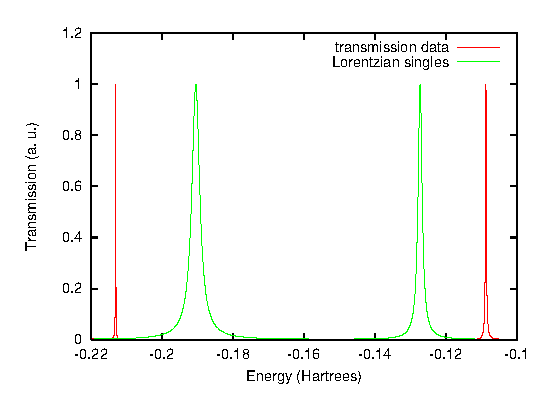
\includegraphics[width=0.9\linewidth]{figures/singles}
	\end{center}
	\caption{}
	\label{fig:singles}
\end{figure}

Finally, we start adding correlation:

\begin{figure}
	\begin{center}
		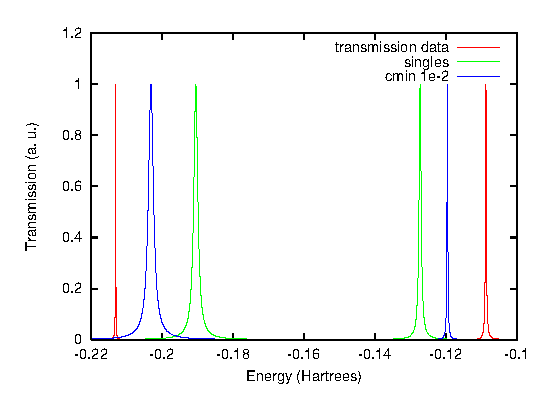
\includegraphics[width=0.9\linewidth]{figures/1em2}
	\end{center}
	\caption{}
	\label{fig:1em2}
\end{figure}

\section{Discussion}
\label{sec:discussion}

